\section{Experimental Results: Comparison and Improvement of Static Analysis Tools}

Our primary experimental results are a set of comparisons of tools using our method, for three languages: Solidity (the most popular language for smart contracts), Java, and Python.  We also use these results to answer a set of research questions that consider the utility of our method:

\begin{itemize}
\item {\bf RQ1:}  Does mutation analysis of static analysis tools produce actionable results?  That is, do raw mutation kills serve to distinguish tools from each other, or are all tools similar in terms of mutation detection capability?
\item {\bf RQ2:}  Does our approach provide additional information beyond simply counting findings for the original, un-mutated analyzed code?  Do \emph{ratios} differ between programs, or does the number of mutants killed simply reflect the ``verbosity'' of each tool?
\item {\bf RQ3:}  Do the rankings that raw kills and ratios establish agree with other sources of information about the effectiveness of the evaluated tools?  Can we confirm results from other evaluation methods, or informal opinion?
\item {\bf RQ4:}  Do mutation scores for clean programs differ from those for programs for which tools report findings before mutation?
\item {\bf RQ5:}  Do individual mutants, prioritized for ease of examination, allow us to identify classes of faults that
 different tools are good at/bad at?  Can we extend this information to improve tools by addressing identified weaknesses?
\item {\bf RQ6:}  How easy is it identify low-hanging fruit for improving tools without prioritization to remove conceptually redundant mutants?
  \end{itemize}

In particular, we consider {\bf RQ2} to be of critical importance; if the mutant ratios for tools differ, then this is clear evidence that our hypothesis that the tendency of mutants to be faults, and to expect that mutated code will, by a sound and precise tool, be flagged as problematic more often than non-mutated code, holds.  This expectation that (some subset of the) mutants can serve as proxies for real, detectable faults is the core concept of our approach.
{\bf RQ4} addresses a concern briefly mentioned in the introduction:  it is possible that warnings for the original code interfere with our definition of detection.  The ideal case for our approach is when a tool report no findings for un-mutated code, and either reports a finding (kills the mutant) or not (does not kill it) when the mutant is introduced.  Chekam et al. showed that the ``clean program assumption'' for testing, the idea that coverage will be similar for faulty and fixed versions of a program, is a threat to the validity of investigations of the relationship between coverage and fault detection \cite{CleanProgram}, and we want to establish that this is unlikely to be the case for our approach.
{\bf RQ5} and {\bf RQ6} receive only preliminary answers, for the smart contract tools.

\subsection{Solidity Smart Contract Tools}

\subsubsection{Smart Contracts and Smart Contract Static Analysis}

Smart contracts are autonomous code instruments, usually operating on a blockchain, that often have critical responsibilities such as facilitating and verifying (large) financial services transactions, tracking high-value physical goods or intellectual property, or even controlling ``decentralized organizations'' with multifarious aspects.  Security and correctness are thus critical in the smart contract domain, and static analysis is a key way to ensure allocation of high-value resources is not compromised.  The most popular smart contract platform, by far, is the Ethereum blockchain, and the Solidity smart contract language \cite{buterin2013whitepaper,wood2014yellow}; the Ethereum cryptocurrency has a market capitalization as we write of over \$15 billion dollars, largely fueled by interest in the smart contract functionality.  Ethereum contracts have been the targets of widely publicized attacks, with large financial consequences  \cite{spank,DAO}.   A recent paper examining results from 23 professional security audits of Solidity contracts argues that effective static analysis is a major key to avoiding such disasters in the future \cite{FC20}.

\subsubsection{Static Analysis Tools Compared}

We analyzed three well-known tools for static analysis of Solidity smart contracts: Slither \cite{slither}, SmartCheck \cite{smartcheck}, and Securify \cite{Securify}.  Slither, based on an SSA-based intermediate language (SlithIR \cite{slither}) is a tool produced by Trail of Bits.  SmartCheck, developed by SmartDec, translates Solidity source directly to an XML-based representation, then uses \emph{XPath} patterns to define problems.  Securify, from SRI Systems Lab at ETH Zurich, works at the bytecode level, first parsing and decompiling contracts, then translating to \emph{semantic facts} in order to look for predefined problems.

\subsubsection{Smart Contract Selection}

We could have used a set of high-transaction contracts, or known-important contracts to validate our approach.  However, we knew that one of our goals in the Solidity experiments was to actually improve a mutation analysis tool, and the developers of the static analysis tools use exactly such benchmarks to validate their tools.  Basing our improvements on mutants of the contracts used for evaluation of proposed detectors would introduce a serious bias in our favor: we would be more likely to produce detectors that would have true positives and few false positives on the benchmark contracts.  We therefore instead selected 100 random contracts for which EtherScan (\url{https://etherscan.io/}) has source code, and used this (quite arbitrary) set of contracts from the actual blockchain to compare tools and identify opportunities for improvement.  The collected contracts had a total of 15,980 non-comment source lines, as measured by {\tt cloc}, with a mean size of 159.8 LOC and a median size of 108 LOC.  The largest single contract had 1,127 lines of code.  Smart contracts are typically smaller than other programs, for various reasons, which explains our use of 100 contracts, compared to a much smaller set of projects for Java and Python.  The Universal Mutator generated 46,769 mutants for the 100 contracts.

\subsubsection{Analysis Results}

\begin{figure}
  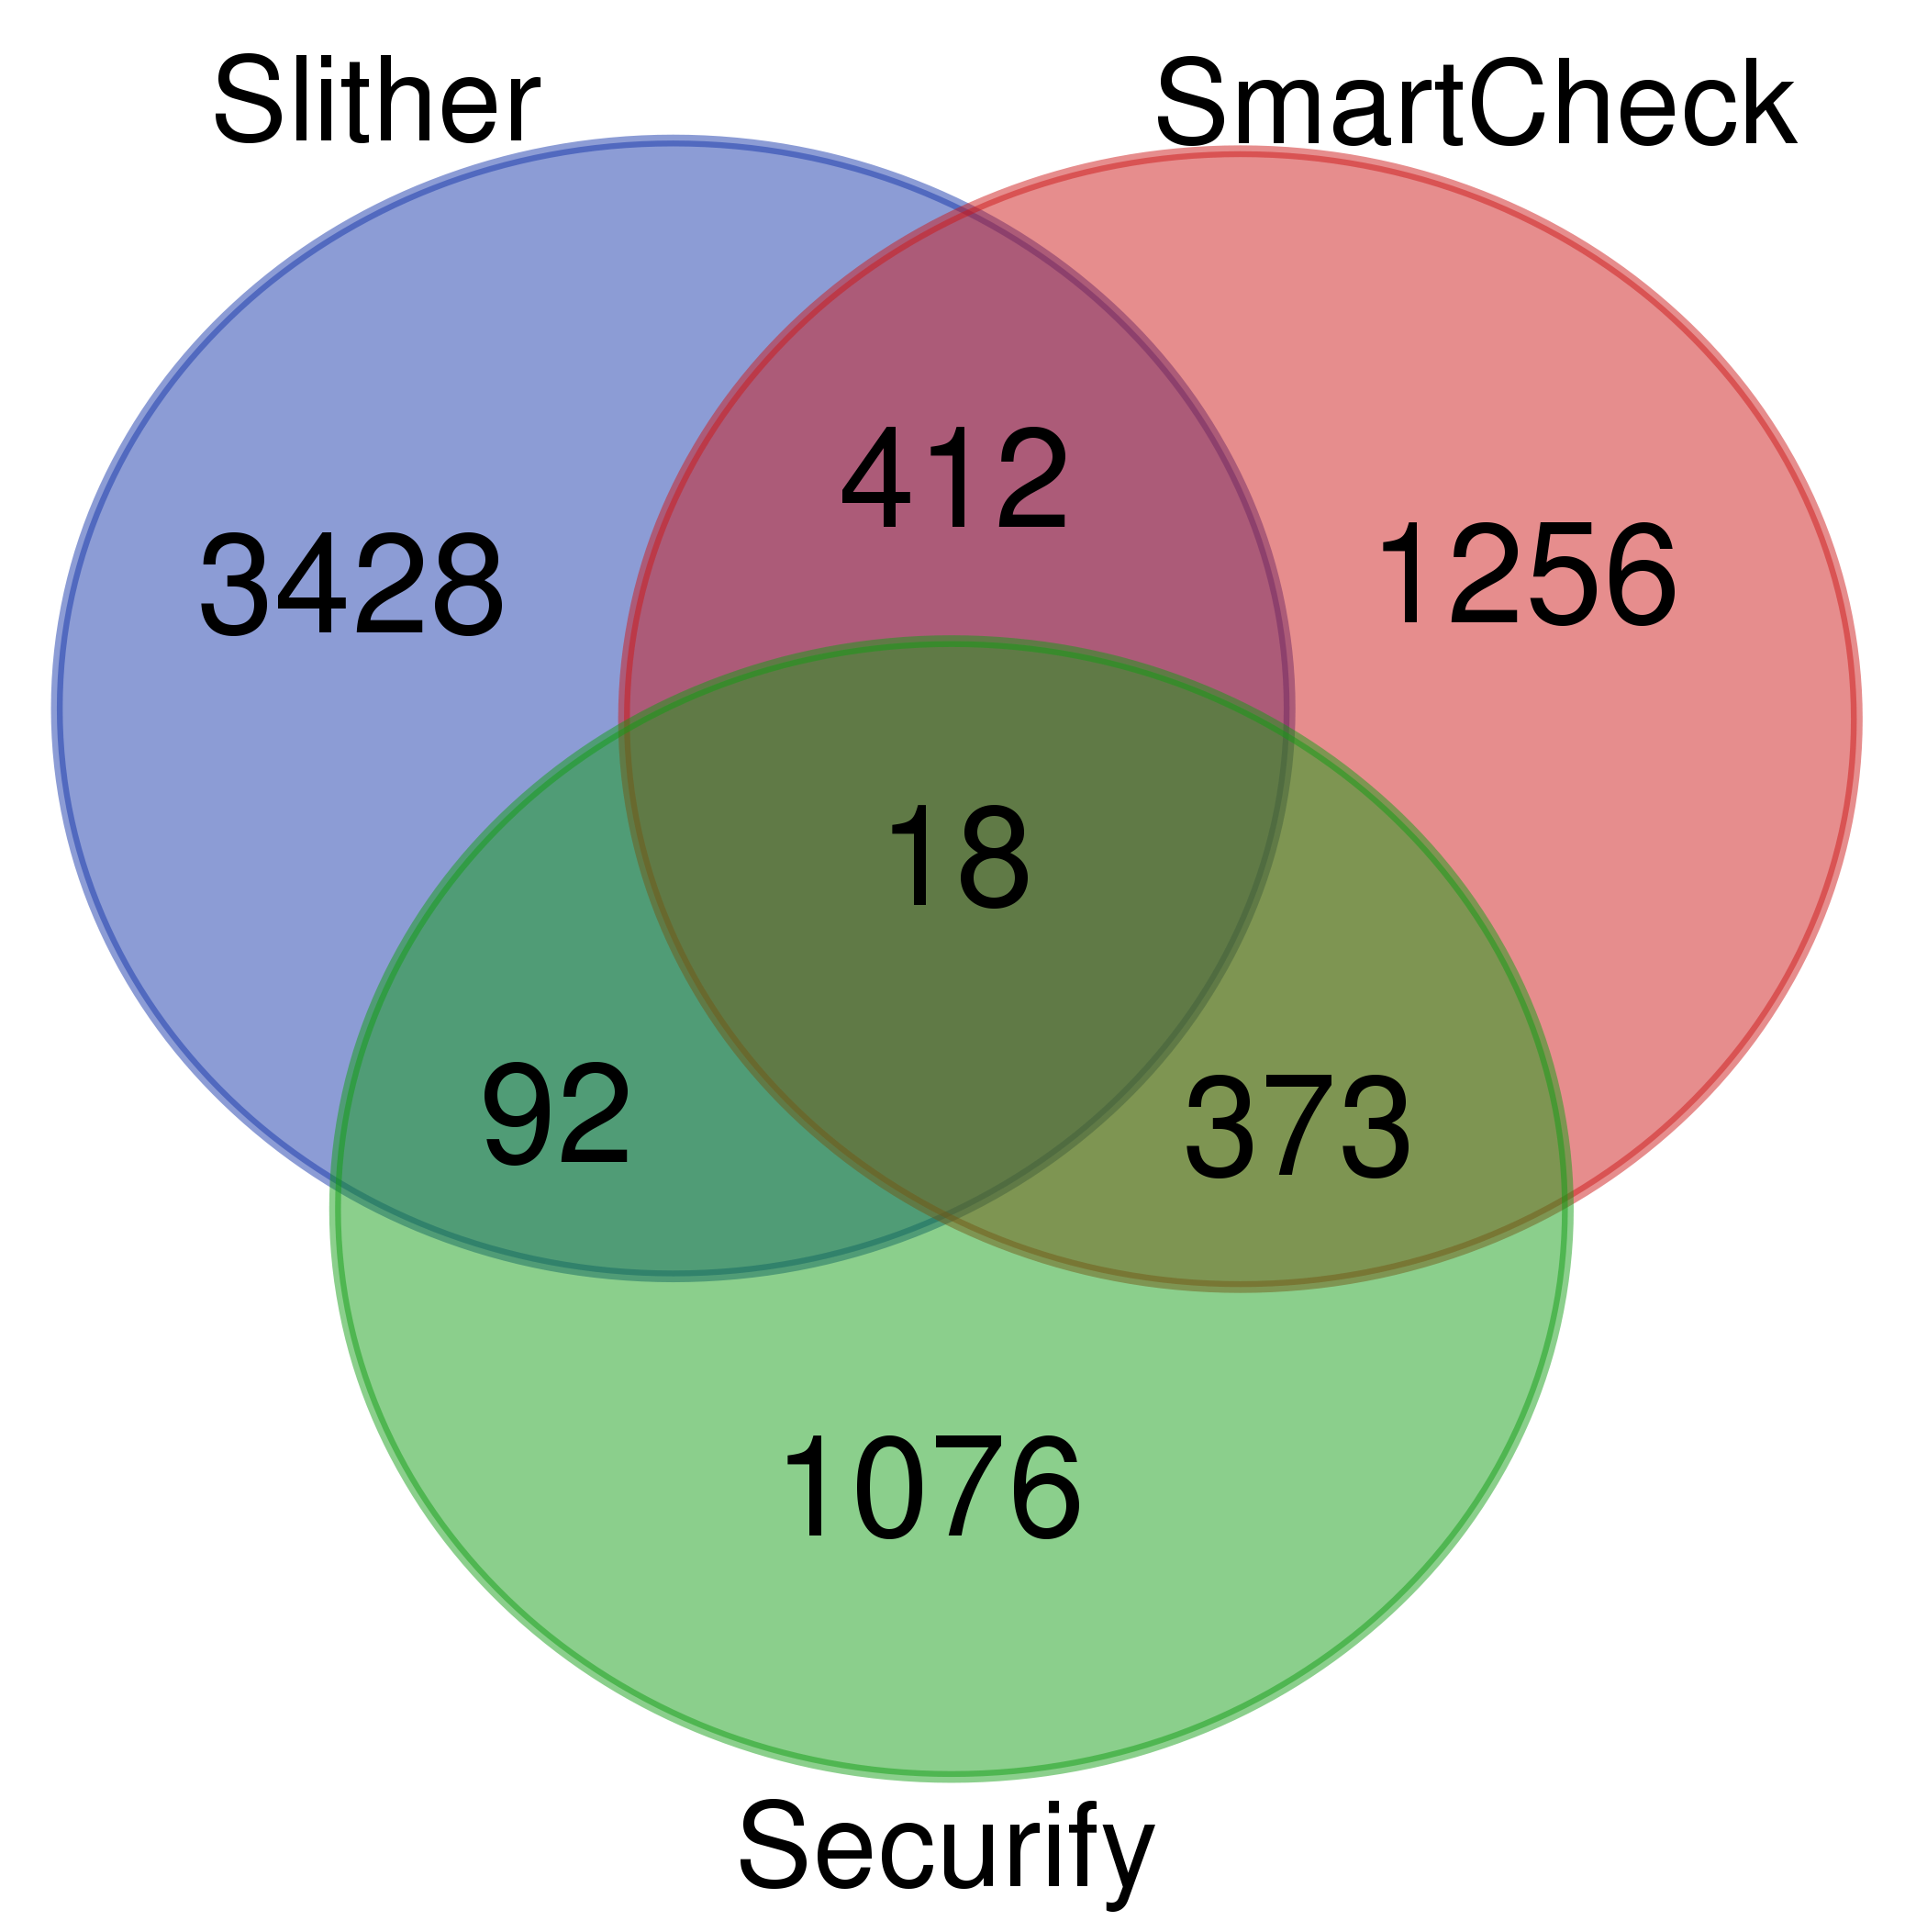
\includegraphics[width=\columnwidth]{solidity.png}
  \caption{Mutants killed by Solidity static analysis tools.}
  \label{fig:solidityvenn}
\end{figure}

\begin{table}
  \begin{tabular}{l|r|r|r|r|r}
    & \multicolumn{2}{|c|}{Findings} & \multicolumn{2}{|c|}{Mutation Score}  & Mutant \\
    Tool & Mean & Median & Mean & Median & Ratio\\
    \hline
    \hline
    Slither & 2.37 & 1.0 & 0.09 & 0.09 & 0.038 \\
    \hline
    SmartCheck & 1.89 & 1.0 & 0.05 & 0.05 & 0.026 \\
    \hline
    Securify & 24.65 & 17.0 & 0.03 & 0.02 &  0.001 \\
    \hline
  \end{tabular}
  \caption{Solidity tools: number of findings and mutation scores over all contracts.}
  \label{tab:scoresolidity}
\end{table}

\begin{table}
  \begin{tabular}{l|r|r|r|r|r}
    & & \multicolumn{2}{|c|}{} & \multicolumn{2}{|c}{Clean For All (3)} \\
    & \# Clean & \multicolumn{2}{|c|}{Mutation Score} &  \multicolumn{2}{|c}{Mutation Score}\\
    Tool & Contracts & Mean & Median & Mean & Median\\
    \hline
    \hline
    Slither & 39 & 0.11 & 0.11 & 0.09 & 0.09 \\
    \hline
    SmartCheck & 27 & 0.03 & 0.01 & 0.03 & 0.00 \\
    \hline
    Securify & 5 & 0.00 & 0.00 & 0.00 & 0.00 \\
    \hline
  \end{tabular}
  \caption{Solidity tools: clean contract counts and mutation scores.}
  \label{tab:cleansolidity}
\end{table}


Figure \ref{fig:solidityvenn} shows the mutants killed by the Solidity analysis tools.  Tables \ref{tab:scoresolidity} and \ref{tab:cleansolidity} provide numeric details of the results, including the \emph{ratio} for each tool, adjusting its mutation scores by its' general tendency to produce findings.  First, a user examining these results would suspect that Slither and SmartCheck are both useful tools, and should likely both be applied in a high-risk security-sensitive context like smart contract development.  Second, a user might suspect that the large number of findings produced, and smaller number of mutants killed, for Securify, mean that including Securify in the static analysis tool stable is a more difficult decision.  On the one hand, Securify does detect nearly as many mutants it alone can identify as SmartCheck.  The large number of findings, and very bad mutant ratio, however, lead us to suspect that many of these ``detected'' mutants are false positives (or, at least, that the problem is not the one Securify identifies).  Extracting the signal from Securify's noise will be difficult.  We also note that while running Slither and SmartCheck on all 46,769 valid mutants was relatively quick (it took about 6 days sequential compute time for Slither and 3 days for SmartCheck), Securify often required many hours to analyze a mutant, and frequently required a few days to analyze a mutant; the full analysis required over three months of compute time.

For our research questions, {\bf RQ1} is clearly answered in the affirmative.  Figure \ref{fig:solidityvenn} shows that the tools address quite different problems, with all tools reporting far more uniquely detected mutants than mutants in common with other tools.  There are only 18 mutants detected by all tools, all of them involving replacement of {\tt msg.sender} (the caller of a smart contract, which may be another smart contract) with {\tt tx.origin} (the original initiator of a sequence of blockchain calls, a ``human'' account).  Use of {\tt tx.origin} is usuallly a bad idea, can lead to incorrect behavior, and may not be relied on to be meaningful at all in future versions of Ethereum (\url{https://ethereum.stackexchange.com/questions/196/how-do-i-make-my-dapp-serenity-proof}).  

{\bf RQ2} is also answered in the affirmative.  Counting findings for un-mutated code might suggest that Securify is the best tool, by a wide margin, but in the context of its near-zero mutant ratio, we must suspect that many of the warnings are false positives.  Slither has the best mutant ratio, but the margin between it and SmartCheck confirms that both tools likely provide value.

For {\bf RQ3}, there are only a few tool comparisons in the literature; this is probably due to the fast-moving nature of the blockchain analysis world; the oldest of these tools' publication dates is 2018.  The most extensive is that of Durieux et al. \cite{durieux2019empirical}.  Slither detected 17\% of known vulnerabilities in their analyis, vs. 11\% for SmartCheck and 9\% for Securify. Slither and SmartCheck were also among the four (out of 9) tools that detected vulnerabilities in the most categories; Securify was not.  The overall recommendation of Durieux et al. was to use a combination of Slither and Mythril \cite{mythril-code} for contract analysis.  Parizi et al. \cite{Parizi} also offer a ranking of tools, and determined that SmartCheck was the most effective, and far more so than Securify; unfortunately, they did not include Slither in their set of evaluated tools.

The Slither paper \cite{slither} also provides an evaluation of all three tools.  Their findings counts differ from ours because of different choices (we threw out merely informational results), but these are unrelated to mutation analysis, in any case.  The evaluation only considered reentrancy faults \cite{SurveyAttacks,FC20} (which are sometimes, but only rarely, introduced by mutants).  For reentrancy, Slither performed best on two real-world large contracts, finding subtle bugs in both, SmartCheck detected the problem in one of the two, and Securify detected neither.  For a dataset of 1,000 contracts, SmartCheck had a high false positive rate (over 70\%) but detected more actual reentrancies (209) than Slither (99) or Securify (6).  On the other hand, Slither's low false positive rate of 11\%  makes its results possibly more useful in practice.  It seems safe to say that 

For {\bf RQ4}, on the changes seen when restricting analysis to clean contracts, Slither did slightly better at detecting mutants when the original contract was clean for Slither, and the other two tools did somewhat worse on contracts for which they reported no findings.  For the three contracts clean for all tools, Slither performed almost exactly as it did over contracts in general, and the other tools performed worse, by about the same margin as they did for their own clean contracts.  For our approach, we only need a week version of the ``clean program assumption'':  the threat is that kills may be under-reported for non-clean programs, due to interference with findings for the original code.  It is not a problem if mutation scores are \emph{worse} for programs where a tool reports no findings for the un-mutated code.  We therefore, for smart contracts, find no threat to our approach arising from the presence of findings on un-mutated code.  We speculate that ``clean'' results for some tools result from contracts where the tool has trouble with the contract code, but does not actually crash; Slither may do better on clean code because it has fewer such failures, and clean contracts are probably generally simpler and easier to analyze.

\subsubsection{Improving Slither {\bf (RQ5 and RQ6)}}


\begin{figure}
  {\scriptsize
\begin{code}
  0x598ab825d607ace3b00d8714c0a141c7ae2e6822\_Vault.mutant.275.sol:
  424contracts/0x598ab825d607ace3b00d8714c0a141c7ae2e6822\_Vault.sol:249
        if (!p.recipient.send(p.amount)) \{  // Make the payment
 ==>          if (true) \{  // Make the payment
        if (true) \{  // Make the payment
      \end{code}
      }
      \caption{Mutant showing {\bf Boolean constant misuse}.}
      \label{fig:boolean}
    \end{figure}

    \begin{figure}
      {\scriptsize
\begin{code}
  0x968815CD73647C3af02a740a2438D6f8219e7534\_TTPresale.mutant.311.sol:
  424contracts/0x968815CD73647C3af02a740a2438D6f8219e7534\_TTPresale.sol:175
        require(nextDiscountTTMTokenId6 >= 361 \&\& nextDiscountTTMTokenId6 <= 391);
 ==>  ...361...==>...0...
        require(nextDiscountTTMTokenId6 >= 0 \&\& nextDiscountTTMTokenId6 <= 391);
      \end{code}
      }
      \caption{Mutant showing {\bf Type-based tautologies}.}
      \label{fig:tautology}      
\end{figure}

\begin{figure}
  {\scriptsize
\begin{code}
  0x534ccee849a688581d1b0c65e7ff317ed10c5ed3\_NametagToken.mutant.480.sol:
  424contracts/0x534ccee849a688581d1b0c65e7ff317ed10c5ed3\_NametagToken.sol:650
        byte char = byte(bytes32(uint(x) * 2 ** (8 * j)));
 ==>  ...*...==>.../...
        byte char = byte(bytes32(uint(x) * 2 ** (8 / j)));
      \end{code}
      }
      \caption{Mutant showing {\bf Loss of precision}.}
      \label{fig:divmul}            
      \end{figure}


Based on the differential mutation analysis, we identified three low-hanging fruit to improve the performance of Slither.  The process was simple.  First, we produced a list of all mutants killed by either SmartCheck or Securify, but not killed by Slither.  We then applied the prioritization method based on the FPF algorithm and the distance metric described in Section \ref{sec:prioritizing}, and examined the mutants in rank order.  Many of the mutants were difficult to identify as true or false positives, absent context.  Some opportunities for enhancement were clear, but seemed likely to require considerable effort to implement without producing a large number of false positives.  For example, Securify often detected when an ERC20 token contract's guard preventing making the special 0x0 address the owner of a contract was removed, and issued the error {\tt Violation for MissingInputValidation}. Detecting such missing guards is probably useful, but formulating a way to do it without producing false positives is non-trivial.  We wanted to show that mutants could identify \emph{useful} but \emph{easy to implement} missing detectors.  Examining the first few mutants, we identified three such, based on mutants killed by either SmartCheck or Securify, or both:

\begin{enumerate}
\item {\bf Boolean constant misuse:}  This detector flags code like {\tt if (true)} or {\tt g(b || true)} (where {\tt g} is a function that takes a Boolean input).  Constant-valued conditionals tend to indicate debugging efforts that have persisted into production code, or other faults; there are almost no circumstances where a conditional should not vary with state or input.  This detector is actually split into two detectors, one for this serious issue, and an informational/stylistic detector that notes that code such as {\tt if (x == true)}, while semantically harmless, is difficult to read.  This problem was easily identified from cases such as the mutant in Figure \ref{fig:boolean}, killed by SmartCheck but not Slither:

\item {\bf Type-based tautologies:}  A type-based tautology is again a case where a Boolean expression has a constant value, but this is not due to misuse of a Boolean constant, but is instead due to the \emph{types} in a comparison.  For example, if {\tt x} is an unsigned integer type, the comparison {\tt x >= 0} is always true and {\tt x < 0} is always false.  This detector is a generalization of the SmartCheck detector \url{https://github.com/smartdec/smartcheck/blob/master/rule\_descriptions/SOLIDITY\_UINT\_CANT\_BE\_NEGATIVE/description\_en.html}, modified to actually compute the ranges of types and identify more general instances of tautological comparisons, e.g. {\tt y < 512} where {\tt y}'s type is {\tt int8}.  Again, the problem was easily identified by mutants killed by SmartCheck but not Slither such as the one in Figure \ref{fig:tautology}.

\item {\bf Loss of precision:}  Solidity only supports integer types.  This means that performing division before multiplication can introduce rounding that is not present when the multiplication is performed first.  This is a fairly important problem, given the frequency with which Solidity code performs financial calculations where maximum precision is desired.  SmartCheck provides a detector for such precision losses \url{https://github.com/smartdec/smartcheck/blob/master/rule\_descriptions/SOLIDITY\_DIV\_MUL/description\_en.html}, which enabled it to detect mutants such as the one shown in Figure\ref{fig:divmul}.
\end{enumerate}      

All three of these detectors were submitted as PRs, vetted over an internal benchmark set of contracts used by the Slither developers to evaluate new detectors, and accepted for release in the public version of Slither.  All three detectors produce some true positives (actual problems, though not always exploitable) in benchmark contracts, have acceptably low false positive rates, and were deemed valuable enough to include as non-informational (medium severity) detectors.  The first mutants in prioritized rank exhibiting the issues, shown above, were the 2nd, 9th, and 12th non-statement-deletion mutants ranked for SmartCheck, out of over 800 such mutants.  Using our prioritization, it was possible to identify these issues by examining fewer than 20 unkilled mutants.  Without prioritization, on average a developer would have to look at more than 200, 80, and 400 mutants, respectively, to find instances of these problems.  

There were 92 separately ranked statement deletion mutants also.  These, however, could all be ignored, as they were almost entirely duplicates related to the missing-return statement detector.  If this detector were not already present as a private Slither detector, it would also be a good candidate for addition to the tool.  Our three submitted detectors were not present as private detectors, and only one (the type-based tautology detector) had even been identified, via a GitHub issue, as a potential improvement (and only in the private version of Slither).  

Examining the first 100 mutants in the unprioritized lists for SmartCheck and Securify, ordered by contract ID and mutant number (roughly source line mutated) we were unable to identify \emph{any} obviously interesting mutants, suggesting that for {\bf RQ6} it is indeed hard to use mutation analysis results without prioritization. A large majority of the mutants we inspected involved either the missing
{\tt return} problem noted in the introduction, or replacing {\tt msg.sender} with {\tt tx.origin}; Slither, of course, has a detector for misuses of {\tt tx.origin}, and we believe (but are not sure) that almost all of the differences with respect to such changes are due to intentional behavior. SmartCheck and Securify tend to identify most (though not all) uses of {\tt tx.origin} as incorrect, while Slither has a more selective rule, intended to reduce false positives.
It is hard to scale our efforts here to a larger experiment, since writing and submitting changes to static analysis tools is always going to be a fairly onerous task, but we believe that our successful addition of new detectors, and the ease of identifying good candidate detectors using mutant prioritization supports a limited affirmative answer to {\bf RQ5} and {\bf RQ6}.

\subsection{Java Tools}

70,825 mutants

\subsubsection{Static Analysis Tools Compared}

\subsubsection{Project Selection}

\subsubsection{Analysis Results}

\begin{figure}
  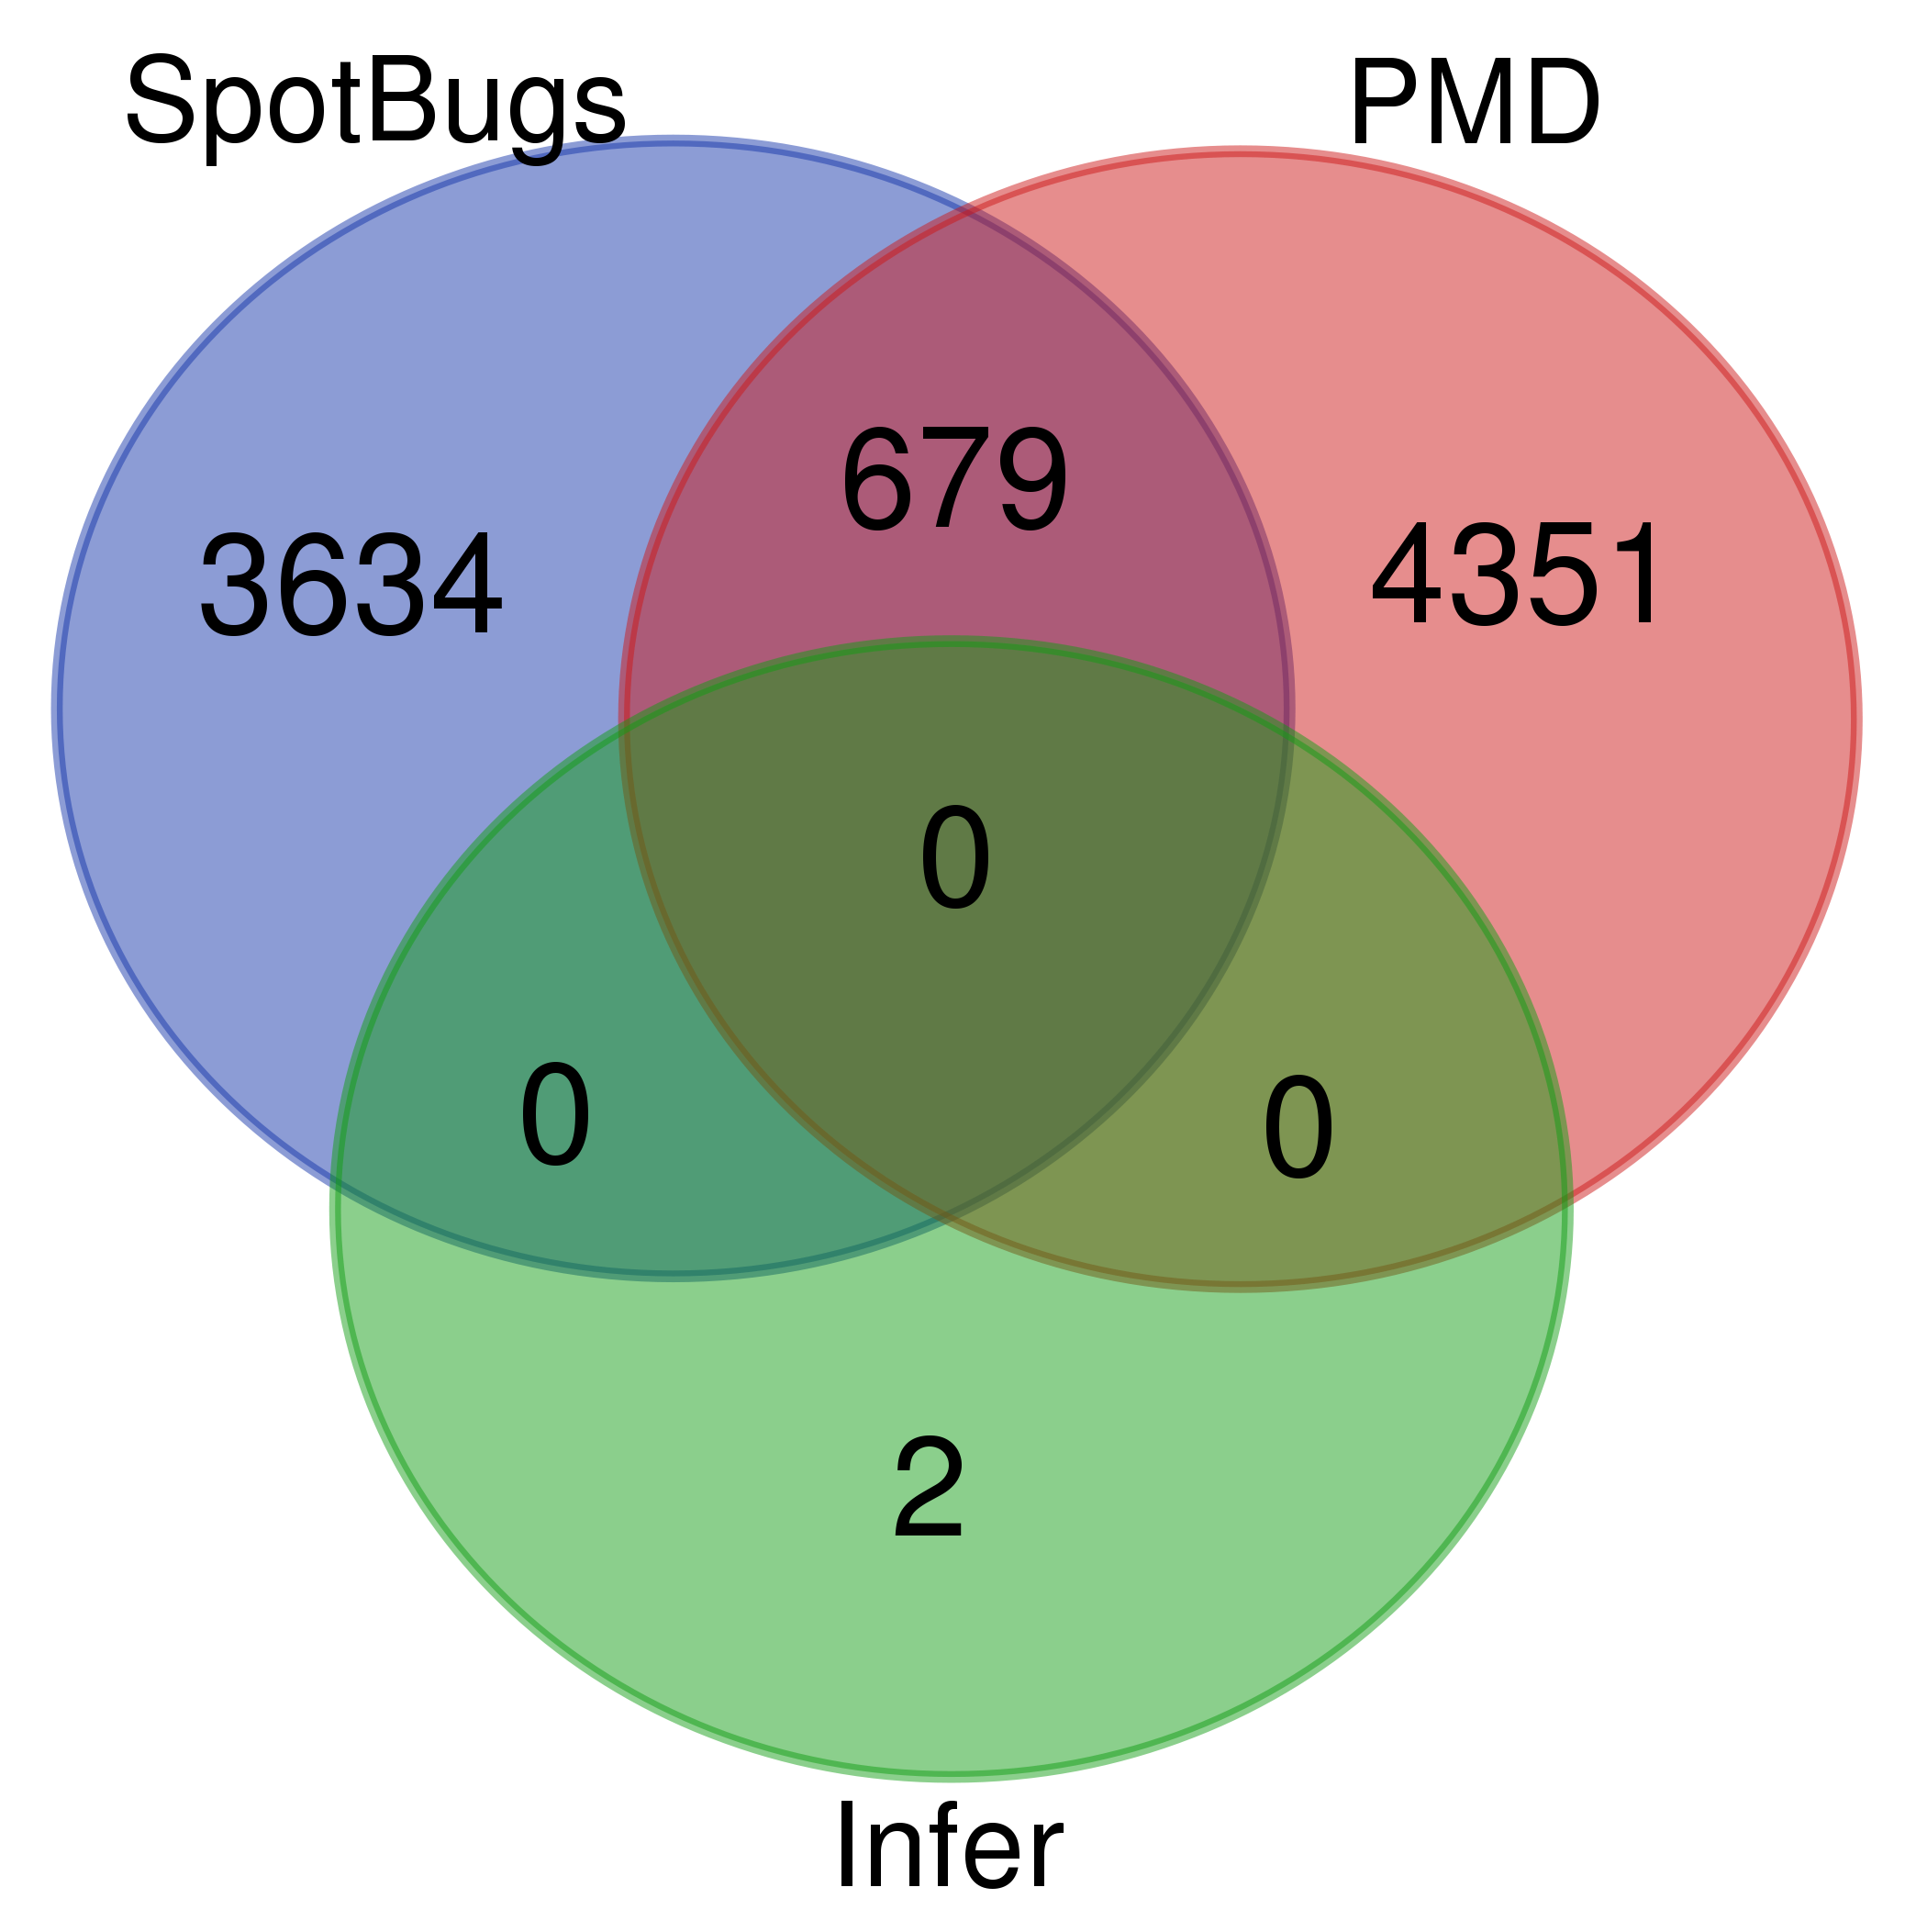
\includegraphics[width=\columnwidth]{java.png}
  \caption{Mutants killed by Java static analysis tools.}
  \label{fig:javavenn}
\end{figure}

\begin{table}
  \begin{tabular}{l|r|r|r|r|r}
    & \multicolumn{2}{|c|}{Findings} & \multicolumn{2}{|c|}{Mutation Score}  & Mutant \\
    Tool & Mean & Median & Mean & Median & Ratio\\
    \hline
    \hline
    SpotBugs & 0.47 & 0.00 & 0.37 & 0.21 & 0.7847 \\
    \hline
    PMD & 1.27 & 0.00 & 0.07 & 0.07 & 0.0562 \\
    \hline
    Infer & 0.07 & 0.00 & 0.00 & 0.00 &  0.0002 \\
    \hline
  \end{tabular}
  \caption{Java tools: number of findings and mutation scores over all projects.}
  \label{tab:scorejava}
\end{table}

\begin{table}
  \begin{tabular}{l|r|r|r}
    & & \multicolumn{2}{|c|}{} \\
    & \# Clean & \multicolumn{2}{|c|}{Mutation Score} \\
    Tool & Projects & Mean & Median \\
    \hline
    \hline
    SpotBugs & 3 & 0.41 & 0.17 \\
    \hline
    PMD & 0 & N/A & N/A \\
    \hline
    Infer & 6 & 0.00 & 0.00 \\
    \hline
  \end{tabular}
  \caption{Java tools: clean project counts and mutation scores.  No projects were clean for all tools, due to PMD producing findings for all projects.}
  \label{tab:cleanjava}
\end{table}

Figure \ref{fig:javavenn} shows the mutants killed by the Java analysis tools.

\subsection{Python Tools}

167,511 mutants

\subsubsection{Static Analysis Tools Compared}

\subsubsection{Project Selection}

\subsubsection{Analysis Results}

\begin{figure}
  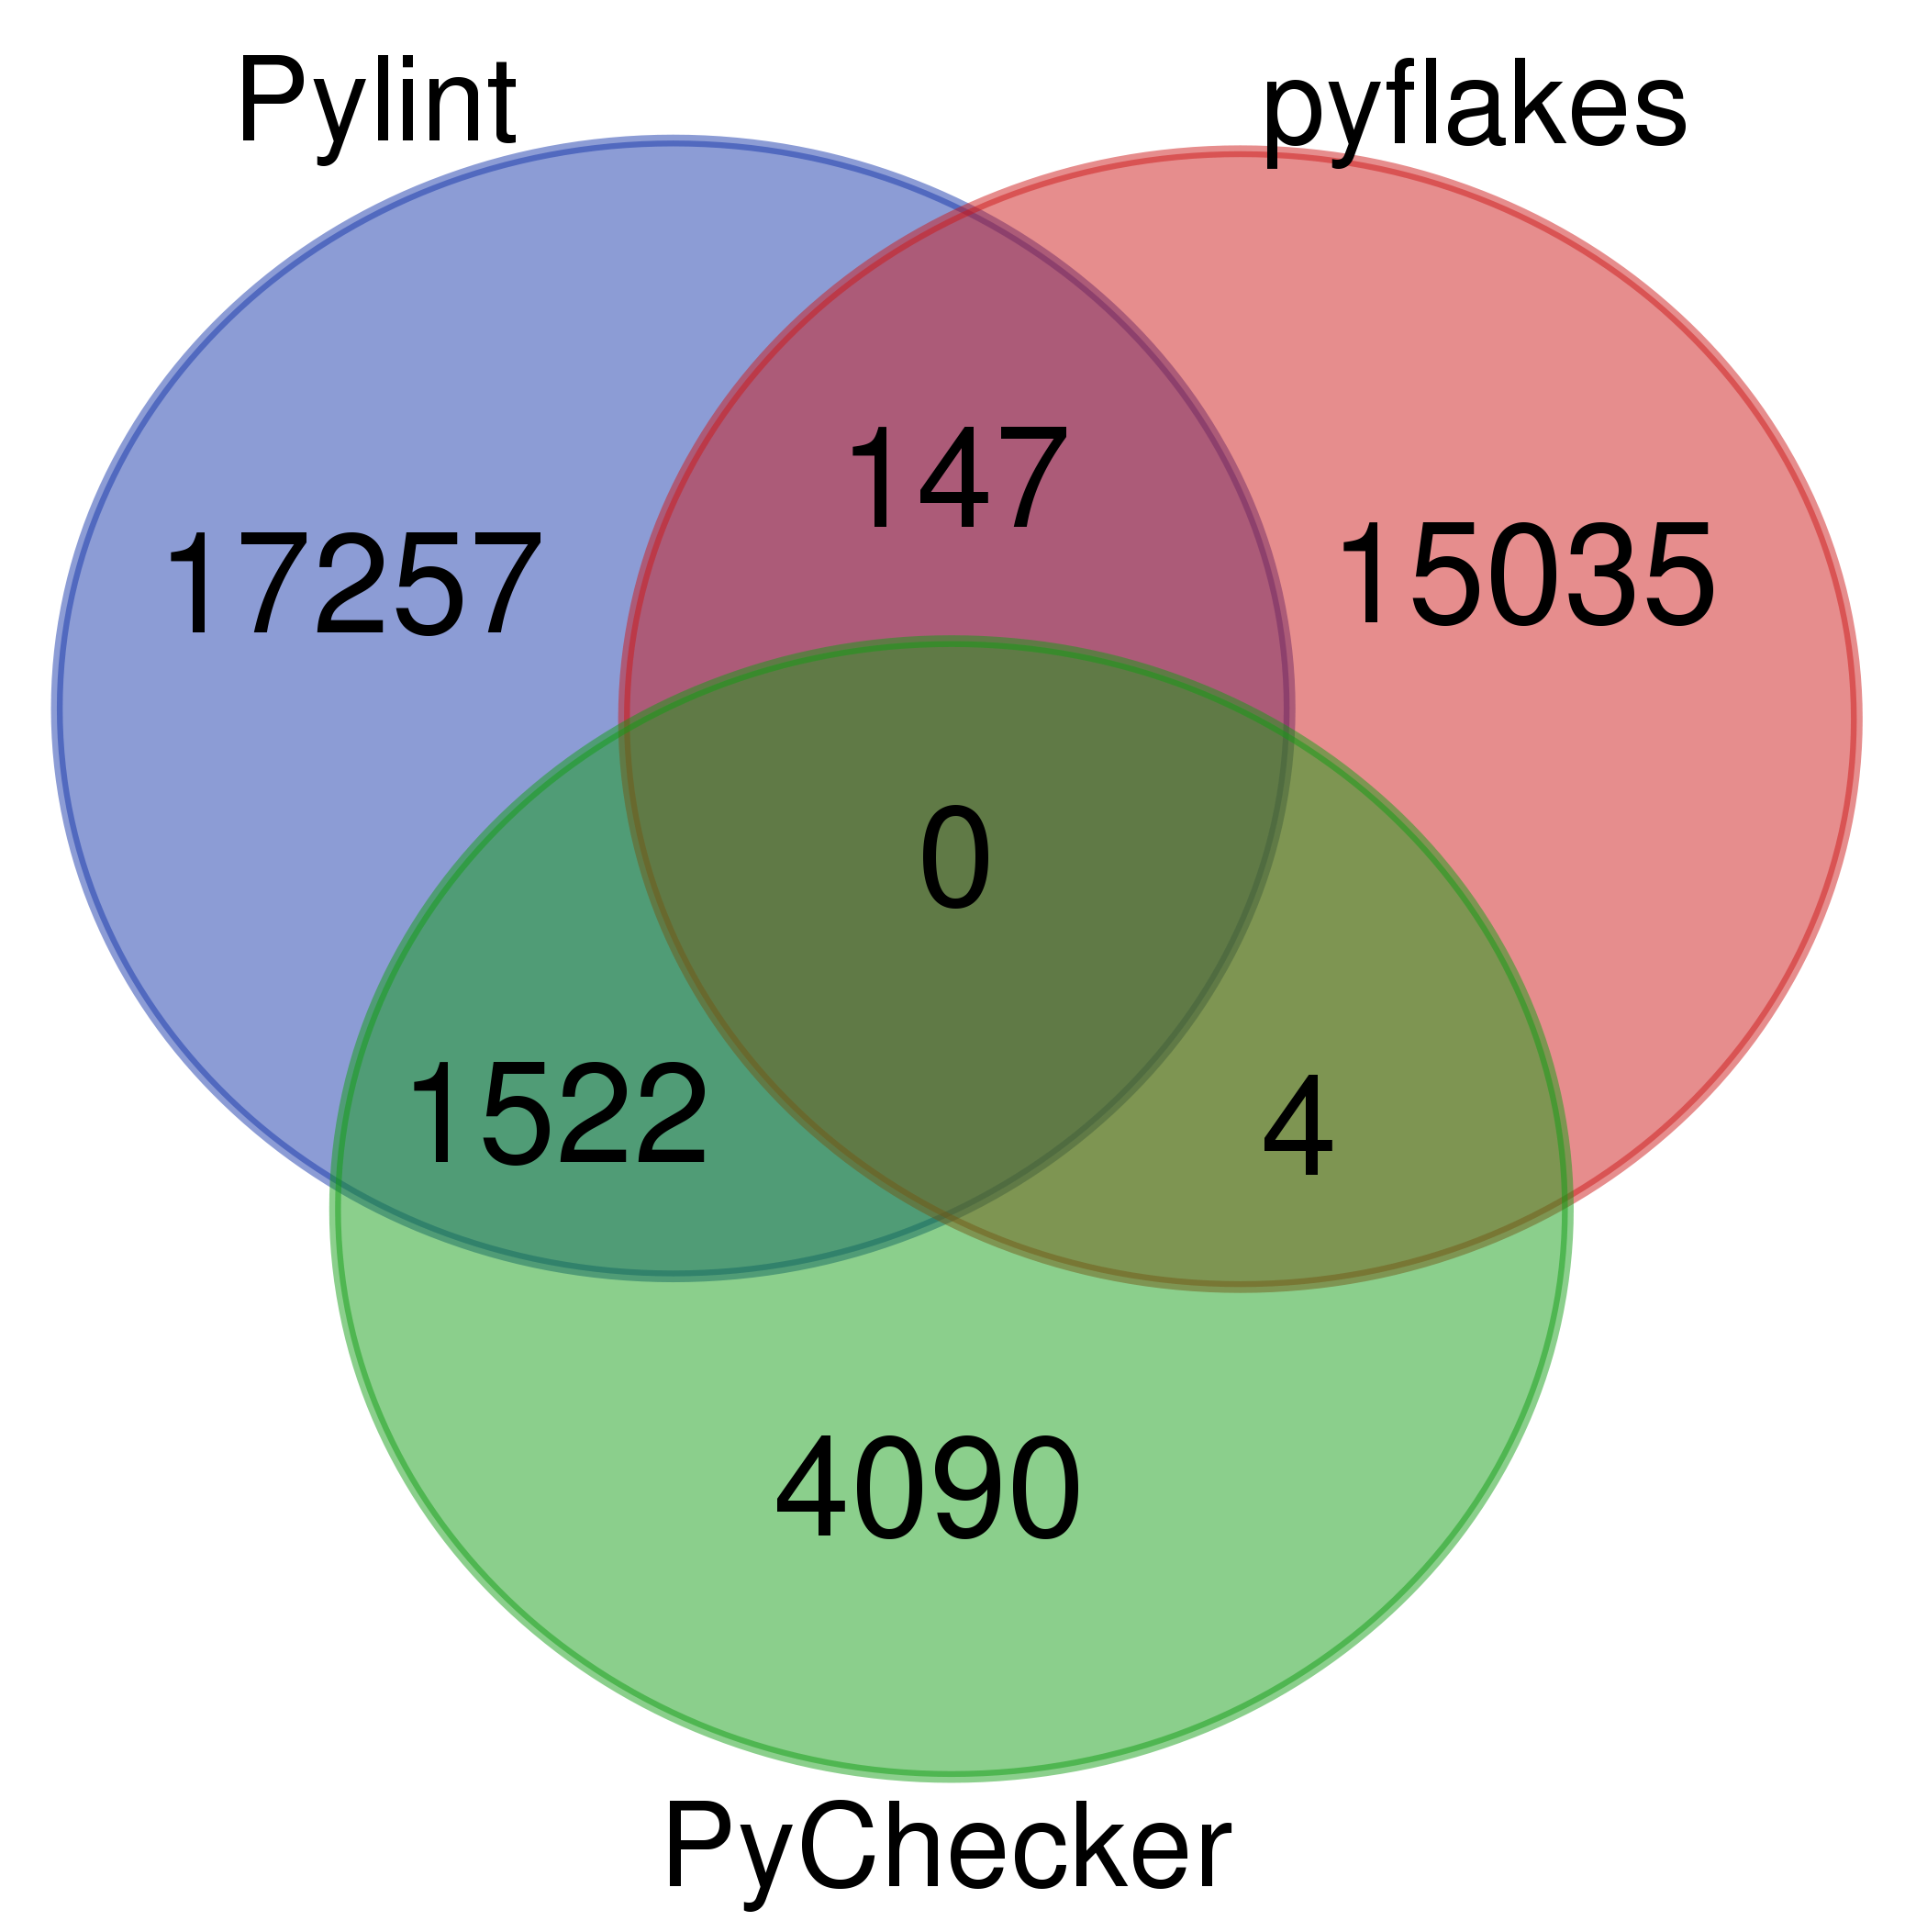
\includegraphics[width=\columnwidth]{python.png}
  \caption{Mutants killed by Python static analysis tools.}
  \label{fig:pythonvenn}
\end{figure}

\begin{table}
  \begin{tabular}{l|r|r|r|r|r}
    & \multicolumn{2}{|c|}{Findings} & \multicolumn{2}{|c|}{Mutation Score}  & Mutant \\
    Tool & Mean & Median & Mean & Median & Ratio\\
    \hline
    \hline
    Pylint & 2.24 & 1.00 & 0.22 & 0.20 & 0.097 \\
    \hline
    pyflakes & 2.4 & 1.00 & 0.03 & 0.00 & 0.012 \\
    \hline
    PyChecker & 0.56& 0.00 & 0.10 & 0.00 &  0.183 \\
    \hline
  \end{tabular}
  \caption{Python tools: number of findings and mutation scores over all projects.}
  \label{tab:scorepython}
\end{table}

\begin{table}
  \begin{tabular}{l|r|r|r}
    & & \multicolumn{2}{|c|}{} \\
    & \# Clean & \multicolumn{2}{|c|}{Mutation Score} \\
    Tool & Projects & Mean & Median \\
    \hline
    \hline
    Pylint & 0 & N/A & N/A \\
    \hline
    pyflakes & 12 & 0.02 & 0.00 \\
    \hline
    PyChecker & 21& 0.01 & 0.00 \\
    \hline
  \end{tabular}
  \caption{Python tools: clean project counts and mutation scores.  No projects were clean for all tools, due to Pylint producing findings for all projects.}
  \label{tab:cleanpython}
\end{table}

\subsection{Threats to Validity}

The primary threat to validity in terms of generalization is that we only examined nine static analysis tools, and our analyses were restricted to 100 smart contracts, 15 Java projects, and 25 Python projects.   Because it is hard to identify a ground truth to compare with (the motivation for our approach), we cannot be certain that our rankings of tools are correct even for these tools and this code.  However, where there are existing discussions of the tools, our results seem to agree with these, but add substantial detail.

A general threat to our approach is that mutants may differ substantially from ``real'' faults, in some way.  This is certainly true, in a sense \cite{GopinathMutants}, but for static analysis purposes, the risk is that some mutation operators align with patterns a particular tool identifies, biasing the evaluation in favor of that tool.  Such faults may be dis-proportionately present in mutants vs. real code.  However, we consider this unlikely.  The vast majority of applied mutation operations for all of our experiments were highly generic, and do not plausibly represent a pattern in which some tool might specialize.  Statement deletions leave no ``trace'' for a tool to match against, but only an omission.  Changing arithmetic and comparison operators and numeric constants (incrementing, decrementing, or changing to 0 or 1) account for most of the non-statement-deletion mutants.  We cannot see how any tool could have a (useful) detection rule that looks for these kinds of changes (a tool obviously would not flag all instances of 0 and 1 constants, or addition).  Finally, many mutants (though many fewer than in these categories) add {\tt break} or {\tt continue} statements.  Again, we do not see how a tool could take advantage of this without either genuinely understanding likely-bad control flow patterns (in which case, we think it ``deserves'' to kill more mutants) or flagging so many instances of these it would have a bad mutant ratio. 